\documentclass[
11pt,%
tightenlines,%
twoside,%
onecolumn,%
nofloats,%
nobibnotes,%
nofootinbib,%
superscriptaddress,%
noshowpacs,%
centertags]%
{revtex4}
\usepackage{ljm}
\usepackage{listings}
\usepackage[utf8]{inputenc}
\usepackage[russian]{babel}

\lstset{
language=C++,
basewidth=0.5em,
xleftmargin=45pt,
xrightmargin=45pt,
basicstyle=\small\ttfamily,
keywordstyle=\bfseries\underbar,
numbers=left,
numberstyle=\tiny,
stepnumber=1,
numbersep=10pt,
showspaces=false,
showstringspaces=false,
showtabs=false,
frame=trBL,
tabsize=2,
captionpos=t,
breaklines=true,
breakatwhitespace=false,
escapeinside={\%*}{*)}
}

\begin{document}

\titlerunning{Meshes self-intersections elimination}
\authorrunning{Freylekhman et al.}

\title{Self-intersections elimination for unstructured surface computational meshes}

\author{\firstname{S.~A.}~\surname{Freylekhman}}
\email[E-mail: ]{freysa@jscc.ru}
\affiliation{Joint Supercomputer Center of the Russian Academy of Sciences -- branch of Scientific Research Institute of System Analysis of the Russian Academy of Sciences, Leninsky prospect 32a, Moscow, 119334, Russia}

\author{\firstname{A.~A.}~\surname{Rybakov}}
\email[E-mail: ]{rybakov@jscc.ru}
\affiliation{Joint Supercomputer Center of the Russian Academy of Sciences -- branch of Scientific Research Institute of System Analysis of the Russian Academy of Sciences, Leninsky prospect 32a, Moscow, 119334, Russia}

\firstcollaboration{(Submitted by TODO)} % Add if you know submitter.
%\lastcollaboration{ }

\received{TODO}

\begin{abstract}
During the numerical solution of the problem of icing a three-dimensional body, the problem arises of representing the surface of this body in the process of an ice buildup formation.
The surface of the streamlined body is described by an unstructured surface computational mesh, the cells of which are triangles.
In the process of icing calculation, the ice buildup can take arbitrary shapes, and the surface mesh must be rebuilt in accordance with this.
At the same time, in reality, situations are not uncommon when individual parts of the ice buildup can connect with each other, layer on each other, forming voids and cavities inside the ice massif.
In the numerical solution, this situation is expressed in the appearance of self-intersections of the surface mesh.
The occurrence of self-intersections of the computational mesh makes it impossible to continue calculations on the surface of the body, so self-intersections must be detected and eliminated.
This work is devoted to a practical algorithm for finding and eliminating self-intersections of an unstructured surface computational mesh in solving the problem of icing a streamlined body.
\end{abstract}

\subclass{65L50} % Enter 2010 Mathematics Subject Classification.

\keywords{icing of a streamlined body, unstructured surface computational mesh, surface rebuilding, self-intersection of the computational mesh, mesh refinement, mesh repairing}

\maketitle

\section{Introduction}

Calculation of icing of a streamlined body surface is an important practical task necessary to ensure the functionality and safety of aircraft \cite{Myers, Farzaneh, Dong, Beaugendre}.
Computer modeling of icing processes can be performed using a wide range of tools, among which are FENSAP-ICE \cite{Bourgault}, LEWICE \cite{Wright}, OpenFOAM \cite{Beld}, AIPAC \cite{Domingos}, IceVision \cite{Aksenov} and others.
The result of the body surface icing calculations are the values of the mass (or volume of ice) accumulated in the different cells of the computational mesh.
In accordance with this information, the surface of the body must be rebuilt in such a way that the new surface reflects the nature and quantitative indicators of the ice buildup.
Rebuilding the surface based on the values of the ice mass in the cells of the computational mesh is usually performed iteratively (the ice buildup is modeled sequentially using separate layers \cite{BourgaultCote, Fortin}).
Special methods of surface smoothing and ice mass redistribution are used to process complex surface areas, depressions and fractures \cite{Thompson, Tong}.

Despite all the efforts used in surface rebuilding, parts of real computational meshes that are used in practical problems can intersect each other during rebuilding.
This corresponds to situations where different parts of the ice buildup collide with each other upon magnification, forming internal cavities.
The intersection of computational meshes generates loops that are hidden under the outer surface, and the presence of such loops makes it impossible to continue the calculations correctly.
Various approaches to the elimination of self-intersections of computational meshes can be found in \cite{Charton, Jung, Skorkovska}.
The main problem faced by the authors of this article in the numerical solution of practical problems was the strongly broken shape of the surface of the formed ice cover and often highly elongated cells of the computational mesh (cells with at least one angle close to zero).
In this article, an attempt was made to give the most simplified algorithm for eliminating self-intersections for such "bad" computational meshes.

\section{General scheme of the algorithm for eliminating self-intersections of the computational mesh}

Before defining the general scheme of the algorithm, let us describe the unstructured surface computational mesh.
The objects of such a mesh are vertices (they are associated with three Cartesian coordinates $x$, $y$, $z$), edges and triangular cells.
In this case, the obligatory conventions are fulfilled: each edge connects exactly two vertices, each triangular cell is incident to three vertices and three edges, and an edge can be incident to at most two cells.
The last requirement allows us to separate the inner and outer regions of the surface formed by a pair of cells that converge in some edge.

\begin{figure}[h]
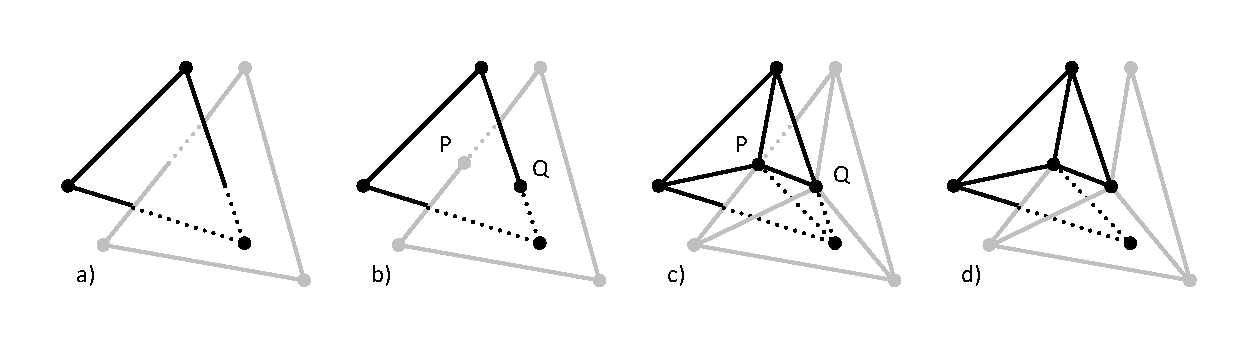
\includegraphics[width=1.0\textwidth]{pics/pic_algorithm_phases_s.pdf}
\captionstyle{center}\caption{Phases of self-intersections elimination.}\label{fig:pic_algorithm_phases_s}
\end{figure}

Fig.~\ref{fig:pic_algorithm_phases_s} shows 4 phases of the intersection elimination algorithm.
At the first phase (fig.~\ref{fig:pic_algorithm_phases_s}, a), all pairs of cells (triangles) that potentially intersect are searched.
In the second phase (fig.~\ref{fig:pic_algorithm_phases_s}, b) all triangles' intersection points are searched (this figure shows the intersection points of $P$ and $Q$).
In the third phase (fig.~\ref{fig:pic_algorithm_phases_s}, c), intersecting triangles are split into smaller ones so that the resulting refined mesh contains only triangles adjacent to edges and vertices (there is no intersections at internal points).
It is obvious that after the execution of the third phase of the algorithm, edges incident to more than two cells can form in the mesh (in fig.~\ref{fig:pic_algorithm_phases_s}, the $PQ$ edge is incident to four cells at once).
Therefore, at the fourth phase of the algorithm (fig.~\ref{fig:pic_algorithm_phases_s}, d), extra mesh cells are removed (sets of cells that form internal mesh cavities are removed).
Next, we consider in more detail each of the above phases of the algorithm separately.

\section{Finding pairs of potentially intersecting triangles}

First, to eliminate self-intersections of the mesh, it is necessary to find all pairs of intersecting (but not adjacent) triangles.
Of course, this issue can be approached directly by considering all $n$ triangles from the computational mesh and performing an intersection analysis of all $\frac{1}{2}n(n - 1)$ pairs.
However, this approach will take a lot of time, since the number of triangles in the computational mesh is large, and the procedure for determining the intersection of two triangles is not trivial.
Let's solve the problem in a different way.

First, instead of pairs of intersecting triangles, we will look for pairs of potentially intersecting triangles.
To do this, we introduce the following concepts.
For triangle $ABC$ let's consider cuboid $[min(A_x, B_x, C_x), max(A_x, B_x, C_x)] \times [min(A_y, B_y, C_y), max(A_y, B_y, C_y) ] \times [min(A_z, B_z, C_z), max(A_z, B_z, C_z)]$ and call it the box of this triangle.
We will say that two triangles potentially intersect if their boxes intersect.
Unlike the intersection of triangles, determining the intersection of rectangular boxes (with sides parallel to the coordinate axes) is a simple operation.
By analogy with the box of a triangle, one can define a box of an arbitrary geometric figure, as well as of a set of such geometric figures.
We will use a box for set of triangles.

Let's build an auxiliary object called a cloud of triangles.
In this cloud, we include all the triangles of the computational mesh.
As an additional data field of the triangle cloud, we will use its box.
Now let's divide the cloud of triangles into two subclouds using a section by an arbitrary plane (fig.~\ref{fig:pic_triangles_cloud_s} shows a two-dimensional illustration of this process).
Each triangle of the original cloud will be assigned to the subcloud that corresponds to that part of the half-space in which the center of the triangle fell.
Thus, for the cloud of triangles under consideration, two child subclouds are formed.
Note that it is not necessary to divide a subcloud into exactly two child subclouds; the number of child subclouds can be arbitrary.
Continuing the process of dividing the clouds of triangles further, we obtain a structure called a cloud tree, at the root of which is the entire set of triangles, and in the leaves -- individual triangles.

\begin{figure}[h]
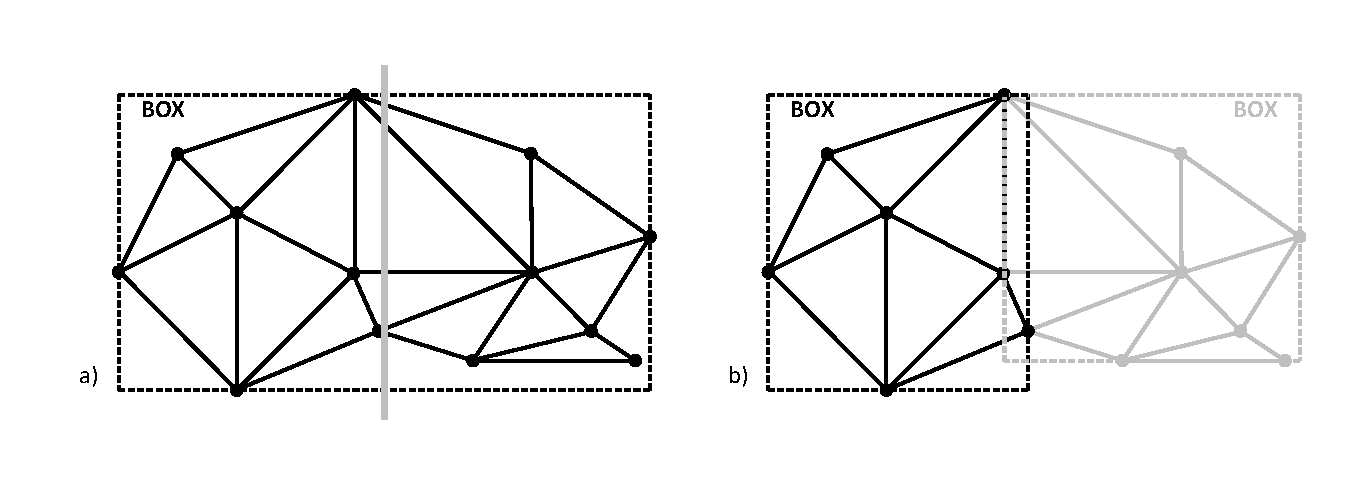
\includegraphics[width=1.0\textwidth]{pics/pic_triangles_cloud_s.pdf}
\captionstyle{center}\caption{Forming of a triangles cloud.}\label{fig:pic_triangles_cloud_s}
\end{figure}

With the help of the formed auxiliary tree of triangle clouds, we can quickly find potentially intersecting triangles.
To do this, it suffices to use the following fact: if two clouds of triangles $T_1$ and $T_2$ are not potentially intersecting (that is, their boxes do not intersect), then any two triangles $t_1 \in T_1$ and $t_2 \in T_2$ are not potentially intersecting.
When using a tree-like search for potentially intersecting triangles using nested triangle cloud boxes, the time it takes to search through all the triangles in the set changes from linear to logarithmic, which greatly speeds up the calculations.

\section{Finding triangle intersection points}

After all pairs of potentially intersecting triangles have been determined, it is necessary to determine their intersection points.
Note the following fact: if two triangles intersect in space, then at least one side of one triangle must intersect the other triangle.
In other words, all intersection points of two triangles cannot be both interior points of one triangle and interior points of a second triangle.
Therefore, the problem of finding the intersections of two triangles is reduced to the problem of the intersection of one triangle with the sides of the second one (and vice versa).

Based on this simple fact, to determine all points of intersection of triangles, it is enough to solve the following particular problems: establishing the fact that two vertices coincide (fig.~\ref{fig:pic_intersection_s}, a), establishing the fact that a point lays inside a segment (fig.~\ref {fig:pic_intersection_s}, b), establishing the intersection of two segments in space (fig.~\ref{fig:pic_intersection_s}, c), establishing the fact of the intersection of a segment with a triangle (fig.~\ref{fig:pic_intersection_s}, d).

\begin{figure}[h]
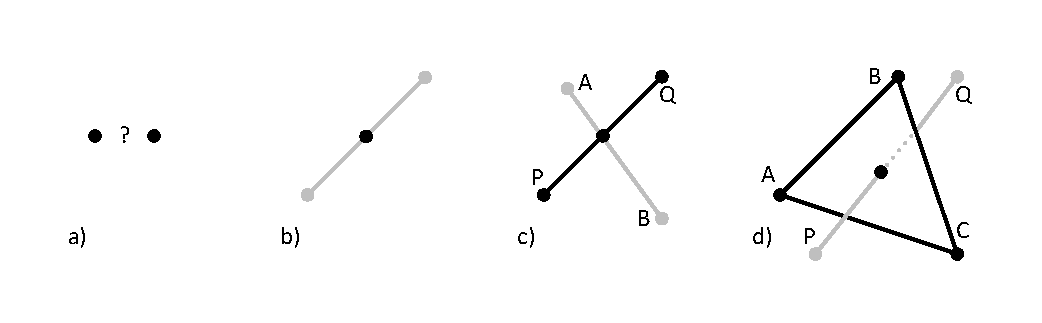
\includegraphics[width=1.0\textwidth]{pics/pic_intersection_s.pdf}
\captionstyle{center}\caption{Search for intersection points of different geometric primitives.}\label{fig:pic_intersection_s}
\end{figure}

Of the above particular problems, only the last two deserve attention.
To solve them, we will use the representation of geometric objects in the form of the locus of points, namely: the segment $PQ$ in space will be represented as the locus of points $P + \phi(Q - P), 0 \le \phi \le 1$ , and the triangle $ABC$ in space will be written as $A + \alpha(B - A) + \beta(C - A), \alpha \ge 0, \beta \ge 0, \alpha + \beta \le 1$ (record data are understood in vector form).

Then, to find intersections of two segments $AB$ and $PQ$ in space, it suffices to solve the following system:

\begin{equation}
\begin{cases}
A_x + \psi(B_x - A_x) = P_x + \phi(Q_x - P_x) \\
A_y + \psi(B_y - A_y) = P_y + \phi(Q_y - P_y) \\
A_z + \psi(B_z - A_z) = P_z + \phi(Q_z - P_z) \\
0 \le \psi \le 1 \\
0 \le \phi \le 1
\end{cases}
\end{equation}

A given system may have no solutions, exactly one solution, or infinitely many solutions.
The case of an infinite number of solutions deserves attention.
In this case, we are dealing with the imposition of two segments on top of each other, and the problem of finding intersections is reduced to the tasks of determining the coincidence of two points and determining whether a point lays inside a segment.

To search for intersections of the triangle $ABC$ with the segment $PQ$, it is necessary to solve the following system of equations:

\begin{equation}
\begin{cases}
A_x + \alpha(B_x - A_x) + \beta(C_x - A_x) = P_x + \phi(Q_x - P_x) \\
A_y + \alpha(B_y - A_y) + \beta(C_y - A_y) = P_y + \phi(Q_y - P_y) \\
A_z + \alpha(B_z - A_z) + \beta(C_z - A_z) = P_z + \phi(Q_z - P_z) \\
\alpha \ge 0 \\
\beta \ge 0 \\
\alpha + \beta \le 1 \\
0 \le \phi \le 1
\end{cases}
\end{equation}

A given system may have no solutions, have exactly one solution, or have an infinite number of solutions.
In this case, the situation of an infinite number of solutions also requires special processing, in which the problem is reduced to determining the intersection points of two segments.

After searching for intersections of all geometric objects, it is necessary to place the found intersection points on the edges of the computational mesh (if the intersection occurred along the edge), or in cells (if the intersection occurred along the internal point of the triangle).
After that, the transition to the next phase of the algorithm is performed.

\section{Splitting triangles into smaller ones}

After the execution of the previous phase of the algorithm, self-intersection points were plotted on some elements of the computational mesh (edges and triangles).
At this phase of the algorithm, it is necessary to refine the mesh in such a way that all such plotted points become nodes of the new refined mesh.
This is the simplest procedure of all steps of the algorithm.
If some plotted point $P$ is inside the triangle $ABC$ (fig.~\ref{fig:pic_split_s}, a), then it is enough to split $ABC \rightarrow ABP, BCP, ACP$ (fig.~\ref{fig: pic_split_s}, b).
If several points fall inside the triangle at once, the partition is performed recursively.
If some plotted point $P$ falls on some edge $AC$ of triangle $ABC$ (fig.~\ref{fig:pic_split_s}, c), then $ABC \rightarrow ABP, CBP$ must be split.
In this case, if the edge $AC$ is not the boundary of the computational mesh, then it is incident to another triangle, which must also be split along this point $P$ (fig.~\ref{fig:pic_split_s}, d).

\begin{figure}[h]
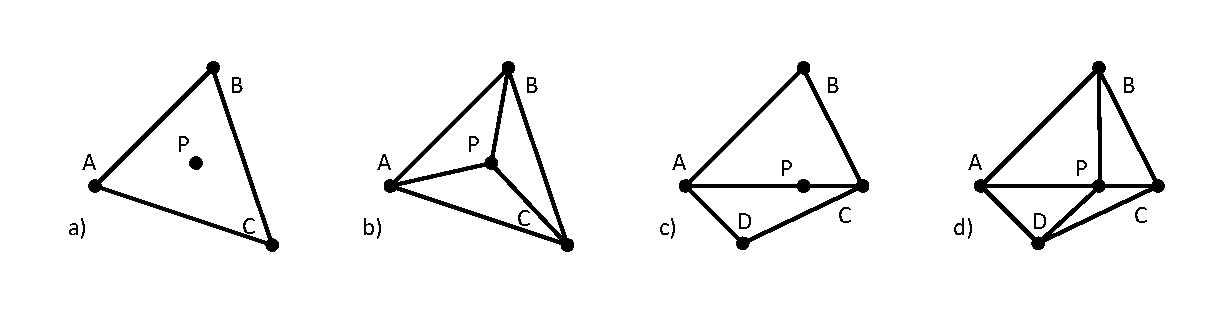
\includegraphics[width=1.0\textwidth]{pics/pic_split_s.pdf}
\captionstyle{center}\caption{Splitting of triangles by intersection points.}\label{fig:pic_split_s}
\end{figure}

It should be noted that with this approach, triangles with angles close to zero may appear.
In order for the quality of the mesh not to decrease significantly, such triangles should be disposed of.
For example, if the point $P$ inside the triangle $ABC$ is too close to the side $AC$ (fig.~\ref{fig:pic_split_s}, a), then the angle $\angle APC$ will be close to 180 degrees, and in this In this case, to preserve the grid quality, it is expedient to move the point $P$ to the side $AC$.

\section{Удаление лишних ячеек}

\begin{figure}[h]
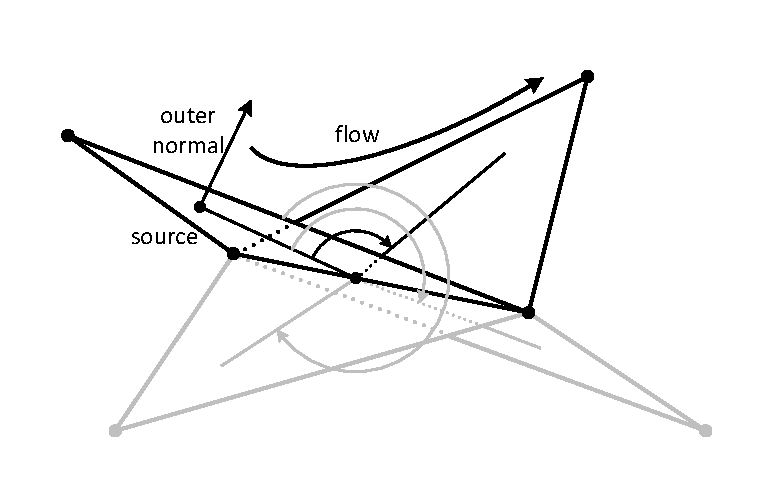
\includegraphics[width=0.7\textwidth]{pics/pic_del_extra_s.pdf}
\captionstyle{center}\caption{Удаление лишних ячеек.}\label{fig:pic_del_extra_s}
\end{figure}

Последним шагом алгоритма является удаление лишних ячеек после измельчения сетки.
В местах самопересения сетки после ее измельчения образуются ребра, которые могут быть инцидентны более чем двум ячейкам (в классическом случае это 4 ячейки, как показано на рис.~\ref{fig:pic_del_extra_s}).
При этом для корректного представления поверхности требуется, чтобы данное ребро было инцидентно только двум ячейкам (остальные ячейки относятся к скрытой области самопересечения и описывают полость, которая должна быть вырезана).

Для определения лишних ячеек необходимо уметь идентифицировать хотя бы одну ячейку, которая точно относится к поверхности (на рис.~\ref{fig:pic_del_extra_s} для такой ячейки обозначена внешняя нормаль).
Этого можно достичь путем обхода поверхности из области, где точно отсутствуют самопересечения.
То есть, если известно, что какая-то ячейка расчетной сетки точно относится к поверхности и одна имеет ровно одну смежную ячейку по некоторому ребру, то эта смежная ячейка также относится к поверхности (однозначно определяется с какой на какую ячейку осуществляется перетекание потока).
Выполняя обход таким образом рано или поздно мы либо обойдем все ячейки (тогда самопересечений нет и сетку корректировать не надо), либо придем к ребру через которое нельзя однозначно определить перетекание потока (как показана на рис.\ref{fig:pic_del_extra_s}).
Для таких ребер будем поступать следующим образом.
Ячейку, про которую точно известна ее принадлежность поверхности, будем называть "хорошей".
В качестве второго претендента на принадлежность к поверхности выберем ту ячейку, для которой угол поворота хорошей ячейки в направлении внешней нормали хорошей ячейки до совпадения будем минимальным.

\section{Заключение}

\begin{figure}[h]
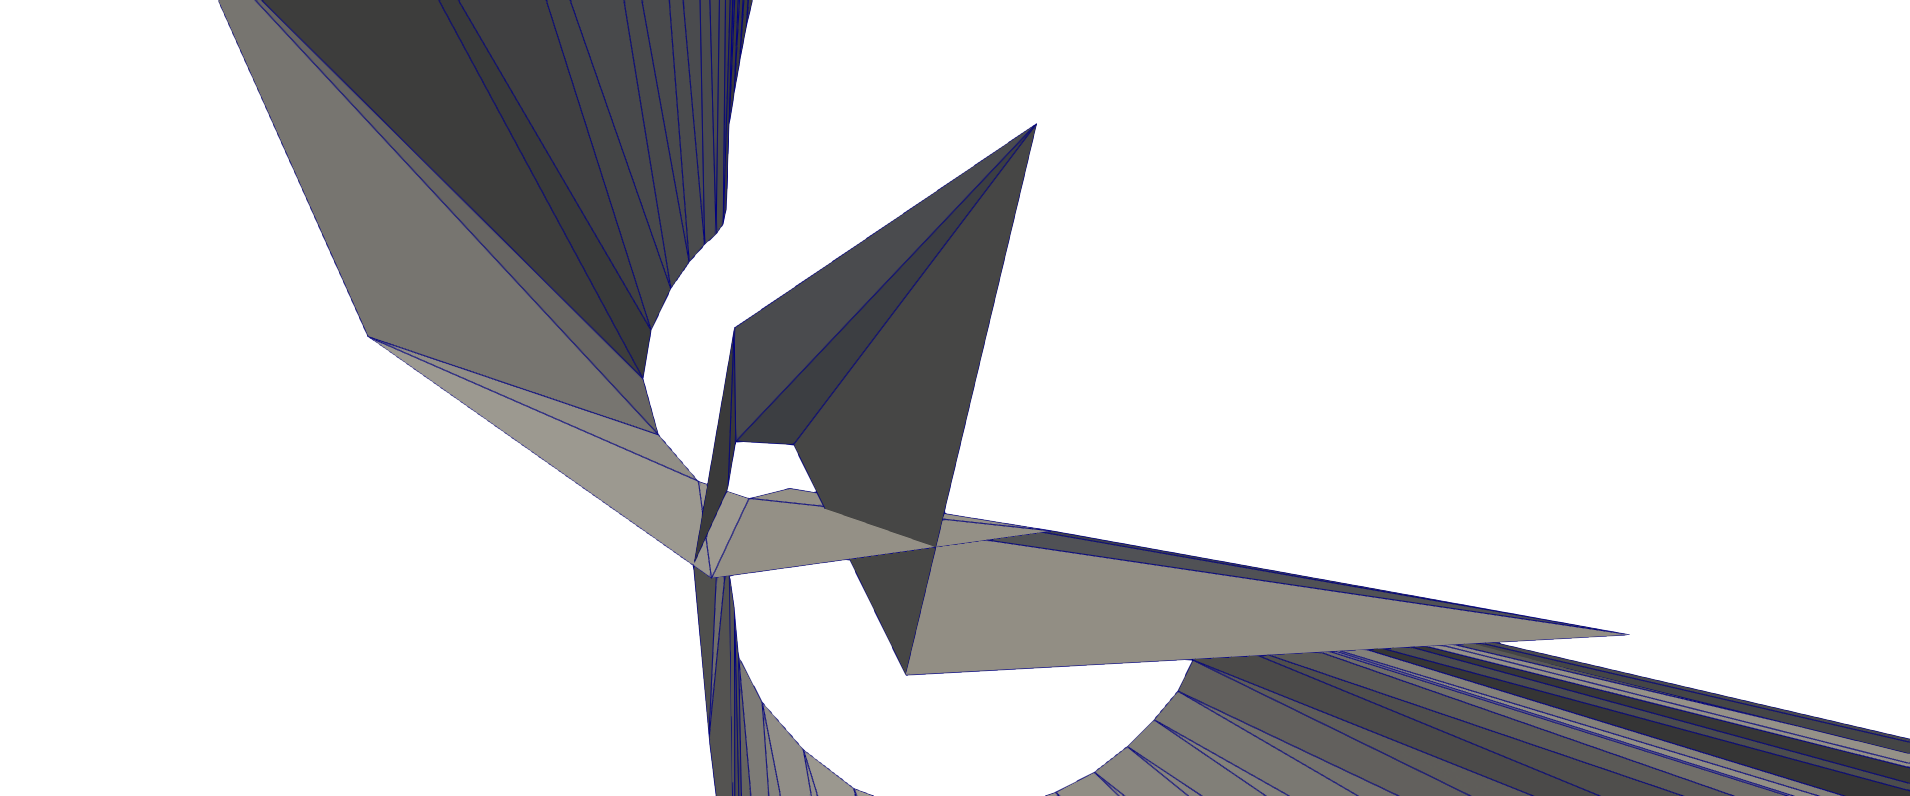
\includegraphics[width=1.0\textwidth]{pics/pic_example_before.png}
\captionstyle{center}\caption{Пример расчетной сетки с самопересечением.}\label{fig:pic_example_before}
\end{figure}

\begin{figure}[h]
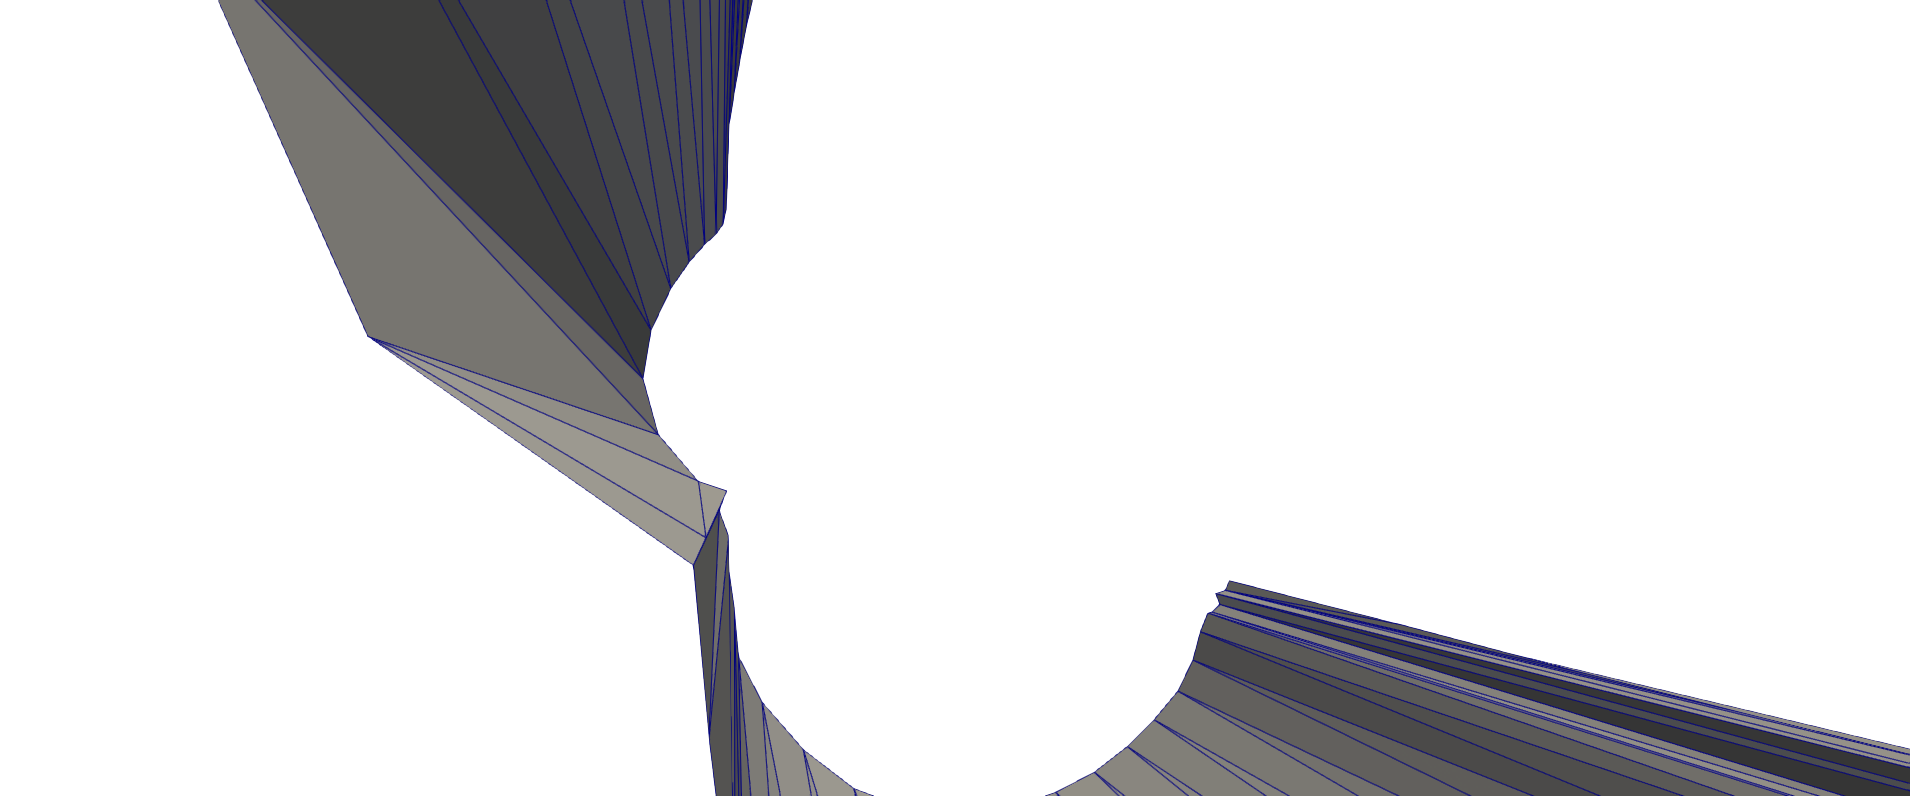
\includegraphics[width=1.0\textwidth]{pics/pic_example_after.png}
\captionstyle{center}\caption{Результата устранения самопересечения.}\label{fig:pic_example_after}
\end{figure}

\begin{acknowledgments}
TODO
\end{acknowledgments}

\begin{thebibliography}{99}

% ice accretion task

\bibitem{Myers}
\refitem{article}
T.~Myers, \textquotedblleft Extension to the Messinger model for aircraft icing,\textquotedblright \ AIAA J. \textbf{39}, 211--218 (2001).

\bibitem{Farzaneh}
\refitem{article}
P.~Farzaneh and G.~Bouchard, \textquotedblleft Modeling a water flow on an icing surface,\textquotedblright \ in \textit{Proceedings of the International Workshop on Atmospheric Icing of Structures IWAIS XI, Montr\'eal, 2005}.

\bibitem{Dong}
\refitem{article}
W.~Dong, J.~Zhu, and X.~Min, \textquotedblleft Calculation of the heat transfer and temperature on the aircraft anti-icing surface,\textquotedblleft \ in \textit{Proceedings of the 27th International Congress of the Aeronautical Sciences, 2010}.

\bibitem{Beaugendre}
\refitem{misc}
H.~Beaugendre, \textquotedblleft A PDE-based approach to in-flight ice accretion,\textquotedblright \ PhD Thesis (Dep. of Mech. Eng., McGill Univ., Montr\'eal, Qu\'ebec, 2003).

% ice accretion software

\bibitem{Bourgault}
\refitem{article}
Y.~Bourgault, H.~Beaugendre, and W.~Habashi, \textquotedblleft Development of a shallow-water icing model in FENSAP-ICE,\textquotedblright \ J. Aircraft \textbf{37}, 640--646 (2000).

\bibitem{Wright}
\refitem{article}
W.~Wright, P.~Struck, T.~Bartkus, and G.~Addy, \textquotedblleft Recent advances in the LEWICE icing model,\textquotedblright \ SAE Int. Technical Paper (2015).

\bibitem{Beld}
\refitem{misc}
E.~Beld, \textquotedblleft Droplet impingement and film layer modeling as a basis for aircraft icing simulations in OpenFOAM,\textquotedblright \ Internship Report (Eng. Fluid Dynamics Department, Univ. Twente, 2013).

\bibitem{Domingos}
\refitem{article}
R.~Domingos and S.~Silva, \textquotedblleft 3D computational methodology for bleed air ice protection system parametric analysis,\textquotedblright \ SAE Int. technical paper (2015).

\bibitem{Aksenov}
\refitem{article}
A.~A.~Aksenov, P.~M.~Byvaltsev, S.~V.~Zhluktov, K.~E.~Sorokin, A.~A.~Babulin, and V.~I.~Shevyakov, \textquotedblleft Numerical simulation of ice accretion on airplane surface,\textquotedblright \ in \textit{Proceedings of AIP Conference, 2019}.

% remeshing

\bibitem{BourgaultCote}
\refitem{article}
S.~Bourgault-C\^ot\'e, K.~Hasanzadeh, P.~Lavoie, and E.~Laurendeau, \textquotedblleft Multi-layer icing methodologies for conservative ice growth,\textquotedblright \ in \textit{Proceedings of 7th European Conference for Aeronautics and Aerospace Sciences EUCASS, 2017}.

\bibitem{Fortin}
\refitem{article}
G.~Fortin, A.~Ilinca, J.-L.~Laforte, and V.~Brandi, \textquotedblleft New roughness computation method and geometric accretion model for airfoil icing,\textquotedblright \ J. Aircraft \textbf{41}, 119--1127 (2004).

\bibitem{Thompson}
\refitem{article}
D.~Thompson, X.~Tong, Q.~Arnoldus, E.~Collins, D.~McLaurin, and E.~Luke, \textquotedblleft Discrete surface evolution and mesh deformation for aircraft icing applications,\textquotedblright \ in \textit{Proceedings of 5th AIAA Atmospheric and Space Environments Conference, 2013}.

\bibitem{Tong}
\refitem{article}
X.~Tong, D.~Thompson, Q.~Arnoldus, E.~Collins, and E.~Luke, \textquotedblleft Three-dimensional surface evolution and mesh deformation for aircraft icing applications,\textquotedblright \ J. Aircraft \textbf{54}, 1--17 (2016).

% self-intersections elimination

\bibitem{Charton}
\refitem{article}
J.~Charton, S.~Baek, and Y.~Kim, \textquotedblleft Mesh repairing using topology graphs,\textquotedblright \ J. of Computational Design and Engineering \textbf{8}, 251--267 (2021).

\bibitem{Jung}
\refitem{article}
W.~Jung, H.~Shin, and B.~K.~Choi, \textquotedblleft Self-intersection removal in triangular mesh offsettings,\textquotedblright \ CAD J. \textbf{1}, 477--484 (2004).

\bibitem{Skorkovska}
\refitem{article}
V.~Skorkovsk\'a, I.~Kolingerov\'a, and B.~Benes, \textquotedblleft A simple and robust approach to computation of meshes intersection,\textquotedblright \ in \textit{Proceedings of the 13th International Joint Conference on Computer Vision, Imaging and Computer Graphics Theory and Applications VISIGRAPP, 2018}.

\end{thebibliography}

\end{document}
